\newcommand\auteur{Tony Clavien, Maxime Guillod, Gabriel Luthier, \& Guillaume Milani}
\newcommand\cours{GEN}
\newcommand\ecole{IL --- TIC --- HEIG-VD}
\newcommand\domaine{Mini-Projet}
\newcommand\titre{Frogger}

\documentclass[a4paper,11pt]{article}
%
\author{\auteur}
\title{\titre}
\date{\today}

\usepackage{fancyhdr}
\usepackage{graphicx}
\usepackage{amsmath}
\usepackage{listings}
\usepackage{listingsutf8}
\usepackage{color}
\usepackage{enumerate}
\usepackage[utf8]{inputenc}
\usepackage[frenchb]{babel}
\usepackage{float}
\usepackage{geometry}
\usepackage{amssymb,mathtools,pifont}
\usepackage{enumitem}
\usepackage{xspace}
\geometry{verbose,tmargin=2.5cm,bmargin=2cm,lmargin=2cm,rmargin=2.5cm}
\selectlanguage{frenchb}
\frenchbsetup{StandardLists=true}
\DeclareGraphicsExtensions{.pdf,.png,.jpg}
\setlength\parindent{0pt}
\setlength{\parskip}{1em}

% headers & footers
\pagestyle{fancy}

\lhead{\domaine}
\rhead{\titre}

\lfoot{\auteur}
\cfoot{}
\rfoot{\thepage}

%%%%%%%%%%%%%%%%%%%%%%%%%%%%%%%%%%%%%%%
%%%%%%% BEGIN DOCUMENT
%%%%%%%%%%%%%%%%%%%%%%%%%%%%%%%%%%%%%%%

\begin{document}
\clearpage\maketitle
\thispagestyle{empty}

	\maketitle
	\begin{figure}[h!]
		\centering
		
\includegraphics[scale=0.7]{../Logo/logo.jpg}
	\end{figure}
	\newpage

	% % Entete première page
	% \thispagestyle{empty}
	% %
	% \noindent \cours \hfill \ecole{} \newline
	% \noindent \auteur \hfill \today \newline
	% \hrule
	% \vspace{7mm}
	% \noindent {\large \bf \domaine } \hfill \titre {\large \bf }\\[3mm]
	% \hrule

	\tableofcontents
	\listoffigures
	\listoftables

	\newpage

	\section{Fonctionnement général}
	\subsection{Objectifs de base}
	Le but de ce projet est de réaliser une application client-serveur dans le cadre du cours GEN. Nous avons décidé de proposer un jeu de type « Frogger » en version valaisanne. \par

	Le but du jeu sera de faire descendre une piste de ski à un Valaisan. Il devra éviter les skieurs genevois la traversant la piste à vive allure.


	\begin{figure}[h!]
		\centering
		\fbox{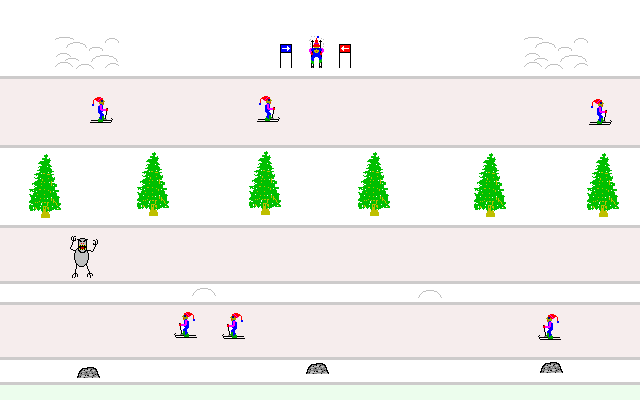
\includegraphics[scale=0.7]{../Screenshots/demo.png}}
			\caption{Maquette d'une partie}
			\label{maquette}
	\end{figure}

	Les zones rouges sont les zones à disposition du joueur 2 pour placer les obstacles, les sapins sont des obstacles fixes. Le joueur 1 gagne s'il atteint la zone en vert sans heurter d'obstacle.

	\subsection{Utilisation de l'applicatif}
	Le joueur 1 contrôle son personnage à l'aide des flèches du clavier ($\leftarrow \downarrow \rightarrow$) et tente d'éviter les obstacles. Le joueur 2 place les obstacles dans les colonnes, ceci fait que l'obstacle se met en mouvement dans la colonne. Une bouteille de Fendant\texttrademark se vide au fur et à mesure que le joueur 2 place des obstacles. Il doit ensuite attendre qu'elle se remplisse à nouveau pour placer de nouveaux obstacles.\par

	L'administrateur peut régler les paramètres du jeu (« skin » du jeu, vitesse des obstacles, vitesse de rechargement de la bouteille de Fendant\texttrademark). L'administrateur est un rôle hérité de celui de joueur (un administrateur est donc avant tout un joueur). Ce droit est stocké dans la base de données.

	\subsection{Règles du jeu}
	Pour le joueur 1: le but est d'arriver en bas de la piste sans avoir heurté d'obstacle. \\
	Pour le joueur 2: le but est que le joueur 1 heurte un obstacle.

	\subsection{Contraintes}
	Le joueur 1 ne peut pas revenir en arrière, une fois descendu une portion de piste il peut s'arrêter, changer de «colonne», continuer à descendre. \par

	Le joueur 2 peut envoyer des obstacles pour autant que la bouteille de Fendant\texttrademark ne soit pas vide.

	\subsection{Priorités de développement}

	\begin{enumerate}
		\item Première version du jeu «standalone» avec un seul joueur qui prend le rôle du joueur 1 (descendre la piste). Les obstacles sont envoyés aléatoirement. (En parallèle, développement du serveur et de l'API).
		\item Ajout du deuxième joueur en local (les deux jouent sur la même machine avec des touches différentes du clavier).
		\item Les joueurs jouent chacun sur leur machine et se connectent à un serveur distant centralisant la partie. Lorsqu'un joueur se connecte, il voit la liste des parties crées (soit en attente d'un joueur, soit en cours). Il peut soit rejoindre une partie en attente d'un joueur soit créer une nouvelle partie.
		\item L'administrateur peut configurer le serveur (paramètres des parties).
	\end{enumerate}

	\subsection{Base de données}
	La base de données stocke et partage les informations suivantes entre les joueurs et l'administrateur :
	\begin{itemize}
		\item Informations des joueurs (nom d'utilisateur, mot de passe, rôle, points totaux gagnés)
		\item Informations des parties (joueurs, points remportés par chacun)
		\item Paramètres de l'application (ce qui peut être configuré par l'administrateur)
		\item Logs de l'application
	\end{itemize}


	\section{Partage des responsabilité serveur --- client}

	\section{Cas d'utilisation}

	\newpage
	\section{Protocole d'échange entre le client et le serveur}
		\subsection{Communication}
			Nous allons utiliser JSON\footnote{JSON : JavaScript Object Notation} comme protocole d'échange entre le client et le serveur. \\
			En effet, de part la structure de son contenu, l'échange d'information entre les deux intervenants est très facilement sérialisable/désérialisable, sans compter sur le fait que le contenu est lisible par un individu (contrairement à un contenu binaire).
		\subsection{Données échangées}

	\section{Ébauche du modèle de domaine}

	\section{Base de donnée}

	\section{Rôle des participants}

	\newpage
	\section{Plan d'itération}
		\begin{enumerate}
			\item Création de l'interface de base
			\item Ajout du 1er joueur avec les obstacles
			\item Ajout du 2ème joueur en local
			\item Mise en place des logiques de jeu
				\subitem Conditions de départ
				\subitem Conditions de victoire
				\subitem Barre de recharge pour la pose d'obstacle
			\item Ajout de la communication avec le serveur
			\item Application administrateur
			\item Ajout du Lobby
			\item Finalisation 
		\end{enumerate}

\end{document}
